\documentclass{llncs}

\usepackage{amsmath}
\usepackage{amssymb}
\usepackage{graphicx}
\usepackage{enumerate}
\usepackage{url}

\newcommand{\tup}[1]{\langle #1 \rangle}
\newcommand{\Omit}[1]{}
\newcommand{\vvec}[1]{\mathbf{#1}}
\newcommand{\join}{\bowtie}
\newcommand{\R}{\mathcal{R}}
\newcommand{\Q}{\mathcal{Q}}
\newcommand{\mcdsat}{\textsc{McdSat}}
\newcommand{\minicon}{{MiniCon}}

\newcommand{\qrule}{:\!\!-}
\newcommand{\orule}{\sqsubseteq}
\renewcommand{\L}{\mathcal{L}}
\newcommand{\M}{\mathcal{M}}

% Ontology concepts
\newcommand{\trip}{\textit{trip}}
\newcommand{\planetrip}{\textit{plane-trip}}
\newcommand{\traintrip}{\textit{train-trip}}
\newcommand{\AAflight}{\textit{AA-flight}}
\newcommand{\UAflight}{\textit{UA-flight}}
\newcommand{\ATtrain}{\textit{AT-train}}
\newcommand{\UPtrain}{\textit{UP-train}}
\newcommand{\flight}{\textit{flight}}
\newcommand{\train}{\textit{train}}
\newcommand{\UScity}{\textit{uscity}}

% Constants
\renewcommand{\AA}{\text{AA}}
\newcommand{\UA}{\text{UA}}
\newcommand{\AT}{\text{AT}}
\newcommand{\UP}{\text{UP}}
\newcommand{\PA}{\text{Paris}}
\newcommand{\NY}{\text{NY}}
\newcommand{\LA}{\text{LA}}
\newcommand{\AL}{\text{AL}}

% Services
\newcommand{\nationalFlight}{\textit{national-flight}}
\newcommand{\onewayFlight}{\textit{one-way-flight}}
\newcommand{\nationalTrain}{\textit{national-train}}
\newcommand{\onewayTrain}{\textit{one-way-train}}
\newcommand{\onestop}{\textit{one-stop}}
\newcommand{\toPA}{\textit{to-pa}}
\newcommand{\onestopPA}{\textit{onestop-to-pa}}
\newcommand{\fromNY}{\textit{from-ny}}
\newcommand{\fromLA}{\textit{from-la}}

\begin{document}

\allowdisplaybreaks
\title{An Expressive and Efficient Solution to the Service Selection Problem}
\author{Daniel Izquierdo \and Mar\'{\i}a-Esther Vidal \and Blai Bonet}
\institute{Departamento de Computaci\'on \\
           Universidad Sim\'on Bol\'{\i}var \\
           Caracas 89000, Venezuela \\
           \url{{idaniel,mvidal,bonet}@ldc.usb.ve}}
\maketitle

\begin{abstract}
Given the tremendous amount of potential Semantic Web 
Services that can be created from online sources by using existing annota- 
tion tools, efficient and scalable approaches to solve the Service Selection 
Problem (SSP) are required. In this paper, we propose a framework that 
is firmly grounded on logic. The framework adopts the Local-As-View 
approach~\cite{levy:bucket} that describes services in terms of concepts in a domain 
ontology. A user request is comprised of a conjunctive query on concepts 
from the domain ontology and a set of preferences; the query expresses 
the abstract concepts that must be combined to solve the query, and 
the preferences are used to rank the solutions. Relations in the domain 
ontology are considered to augment the space of available services. Using 
this representation, the problem of service selection is cast as a problem 
of query rewriting, from the area of integration systems. Then, build- 
ing on related work, we devise an encoding of SSP as a logical theory 
whose models are in correspondence with the service rewritings of the 
user query, and in presence of preferences, whose best models are in cor- 
respondence with the best-ranked valid solutions. Thus, by exploiting 
known properties of modern SAT solvers, we provide an efficient and 
scalable solution to SSP. The approach does not only scale up to large 
instances, as the experimental results show, but is also sound and com- 
plete since, being founded on logic, is amenable to formal analysis.
\end{abstract}                

\section{Introduction}
Existing Web infrastructures support the publication and access to a tremendous 
amount of Web data sources, some of which can be labeled and converted into 
Semantic Web Services by using existing annotation tools like the one proposed 
by Ambite et al. \ \cite{AmbiteISWC09}. Once this huge dataset of Semantic Web 
Services become available, users more than ever will require techniques to 
effectively select the services that meet their requirements. In order to achieve 
this goal, functional and non-functional properties of the services should be 
precisely described, as well as criteria to select and rank the solutions that best
 meet user requests.  
 In this paper, we extend an approach traditionally used in the area of data 
integration to solve the Service Selection Problem. First, concepts from a domain
ontology provide a precise description of the semantics of available sources. These 
descriptions correspond to views on concepts of the domain ontology and follow 
the Local-As-View approach (LAV)~\cite{levy:bucket} . LAV mappings are able to 
scale to service datasets that constantly change, in contrast to Global-As-View definitions 
(GAV), where generic concepts are defined in terms of the available sources and 
cannot be easily modified when sources constantly change. A user request is 
modeled as a conjunctive query on the ontology concepts, and user preferences 
are associated with a cost and constraint the solutions of the query. 
Based on this integration framework, we define the problem of selecting the 
services that best meet the user request, as the problem of enumerating and 
ranking the service rewritings of the user query. Each rewriting is associated 
with a cost equal to the cost of the preferences violated by the rewriting, and 
that a best ranked rewriting is one that has minimum cost among all valid 
rewritings. Knowledge encoded in the domain ontology is used to expand the 
space of rewritings. Thus, our proposed service selection approach is cast into 
the well-known Query Rewriting Problem (QRP) for LAV which is central to 
integration systems and has been shown to be NP-complete~\cite{Ullman00}. 
The QRP consists of a conjunctive query that must be answered in terms of views in 
which the query and the views are described using LAV with abstract relations. 
This problem is important in the context of data integration~\cite{Chen05,JaudoinPRST05}, 
and query optimization and data maintenance~\cite{AfratiLU07,levy:bucket}, and 
several approaches have been defined that scale to a large number of views~\cite{arvelo:aaai06,pods:DuschkaG97,sac:DuschkaG97,levy:bucket,pottinger:minicon}.
 
We propose a solution that extends the recent approach of Arvelo et al.\ \cite{arvelo:aaai06}
which is based on the efficient enumeration of models of a propositional logic 
theory. Similarly, given an instance of SSP, a logical theory is constructed such 
that each model of the theory encodes a valid rewriting; the theory can be con- 
structed in polynomial time from the instance of the SSP. All valid rewritings 
are obtained by enumerating all models of the theory in linear time by using 
off-the-shelf model enumeration solvers such as c2d~\cite{c2d} and Relsat~\cite{relsat}; off-the- 
seft SAT solvers such as Minisat~\cite{minisat} can be used to produce all the minimal 
rewritings. Thus, we exploit known properties of modern SAT solvers that 
implement non-chronological backtacking via clause learning, caching of common 
subproblems and heuristics. we provide an efficient and scalable solution to SSP. 
To summarize the contributions of our work are as follows:
\begin{itemize}
\item Service descriptions as LAV mappings on ontology concepts and user preferences as logic constraints, to provide an expressive description framework.
\item Formalization of SSP as the well-known QRP, and the extension of efficient and scalable existing solutions to exploit the properties of modern SAT solvers to construct a logical theory that encodes an instance of SSP, in a way that the theory models encode the valid rewritings and best models 
correspond to the optimal (best) rewritings.
\item Reduction of the combinatorial search, by efficiently enumerating the models.
\end{itemize}

The paper contains five more sections. The next section defines our approach, 
and illustrates the SSP with typical examples. Section 3 describes our solution 
and system architecture; Section 4 reports our empirical results over different
benchmark problems. Sections 5 summarizes existing approaches; and the paper 
concludes with a final discussion in Section 6.

\section{Service Selection Problem}
We consider service selection problems comprised of the
description $IS$ of the integration framework and of an
user request $R$ over the $IS$.

Our setting is based on the assuption that services are
semantically described in terms of a domain ontology. 
Formally, the integration framework corresponds to a tuple
$IS=\tup{D,S,M}$ where $D$ is the domain ontology, $S$ describes
the available services, and $M$ is the collection of LAV mappings
that define the services in $S$ as views on the ontology $D$. 
On the other hand, the user input $R=\tup{Q,P}$ consists of a
request for composition of services, described as a conjunctive
query $Q$ over the ontology, and a set $P$ of preferences for
the requested composition.

In the following subsections, we describe in detail all the
ingredients making up a service selection problem, and illustrate
the framework with several examples.

\subsection{Domain Ontology}

The domain ontology $D$ is a tuple $\tup{\sigma,A}$ where $\sigma$ is a
\emph{signature} for a logical language and $A$ is a collection of axioms
describing the ontology.
A signature $\sigma$ is a tuple $\tup{R_1^{r_1},\ldots,R_n^{r_n},c_1,\ldots,c_m}$
where each $R_i$ is a relational symbol of arity $r_i$,\footnote{We use
the notation $R^r$ to say that $R$ is a relational symbol of arity $r$.}
and each $c_j$ is a constant symbol.
The set of axioms describe the ontology by defining the relationships
between the ontology relations. % Not sure if talk about Datalog here...
For the present work, we only assume subsumption relationships among
concepts that are expressed with rules of the form:
\begin{equation}
\label{eq:orule}
R(\bar x,\bar y, \bar a)\ \orule\ P(\bar x, \bar b)\,,
\end{equation}
where $R$ and $P$ are predicates in $\sigma$ of appropriate arity,
$\bar x$ and $\bar y$ are lists of variables (repetitions allowed),
and $\bar a$ and $\bar b$ are lists of constant symbols in $\sigma$
(repetitions allowed). All these lists except $\bar x$ can be empty.

Although limited in appearance, rules of this form are quite expressive
as they allow us to specify diverse relationships among predicates.
For example,
\begin{itemize}
\item \textbf{Hierarchy of classes and subclasses} (or types and subtypes):
classes are specified with unary predicates. A subclass relantionship
among two classes is directly specified with a simple rule; e.g., the
rule $\textit{penguin}(x) \orule \textit{bird}(x)$ declares that every
penguin is a bird.
\item \textbf{Subrelations via specialization:} A subrelation of $R^r$
can be specified by constraining another relation $P^s$ ($r<s$). 
For example, the rule:
\begin{equation}
\label{eq:QE2}
\textit{descendant}(\textit{Elizabeth II},x)\ \orule\ \textit{noble}(x)
\end{equation}
tells that any descendant of Queen Elizabeth II is a noble.
\item \textbf{Indirect subsumption:} it is even possible to specify
a subrelation via another seemengly unrelated predicate. For example,
the rule:
\[ \textit{citizen-of}(x,\textit{Montreal})\ \orule\ \textit{lives-in}(x,\textit{Canada}) \]
says that when the second argument of `CitizenOf' is fixed to the
constant `Montreal', the tuples in the relation `CitizenOf' are
contained in the set of tuples in the relation `LivesIn' whose
second component is `Canada'.
\end{itemize}
However, we require that the \emph{dependency graph} for the ontology
to be a \emph{forest of trees}. The dependency graph $G(D)$ is a
labeled directed graph that is constructed as follows: the nodes
are the relational symbols in the signature $\sigma$, and there
is an edge $(R,P)$ in the graph iff there is an rule of the
form \eqref{eq:orule} that is labeled with the \emph{bindings}
induced by the rule. For example, if $\textit{descendant}(x,y)$
and $\textit{noble}(z)$ are two predicates in the signature
and there is the rule \eqref{eq:QE2}, there edge from 
Descendant to Noble is labeled with the bindings
$\{x=\textit{Elizabeth II},y=z\}$.

\subsection{Services and LAV Mappings}

The available services are represented by means of another signature
$S=\tau=\tup{S_1^{s_1},\ldots,S_k^{s_k}}$, called the \emph{services signature},
that consists of relational symbols $S_i$ of arity $s_i$: each such symbol
$S_i$ represents a concrete service in the Semantic Web that ``offers''
some information.

The semantic description of services is expressed following the
LAV paradigm in terms of LAV mappings. These mappings describe the
services in terms of concepts in the domain ontology \cite{Ullman00}:
for each service $S_i$, there is a LAV mapping that describes $S_i$
as a \emph{conjunctive query} on the concepts in the ontology; 
input and output attributes of the service are also distinguished.
For example, a service $S(x,y)$ that returns information about
flights originating at a given US city can be described with the view:
\[ S(\$x,y)\ \qrule\ \flight(x,y), \UScity(x)\,, \]
where $flight^2$ and $uscity^1$ are relational symbols in the
ontology; the symbol \$ denotes that $x$ is an input attribute. 
The semantic interpretation of a mapping like this one enforce the following:
\begin{itemize}
\item the service represented by $S$ provides information in the
      form of tuples $(x,y)$,
\item each tuple $(x,y)$ returned by the service satisfies the rhs
      of the view; i.e., $\flight(x,y)$ and $\UScity(x)$, and
\item the views are not necessarily \emph{complete}; i.e., there may be
      other tuples $(x,y)$ that satisfy the rhs of the view but which
      are not available through the service represented by $S$.
\end{itemize}

The LAV approach is commonly used in integration systems because it permits
the scalability of the system as new services become available \cite{Ullman00}.
Under LAV, the appearance of a new service only causes the addition of a new
mapping describing the service in terms of the concepts in the ontology.
Under GAV, on the other hand, the ontology concepts are semantically described
using views in terms of the sources of information.
Thus, the extension or modification of the ontology is an easy task in GAV as
it only involves the addition or local modification of few descriptions
\cite{Ullman00}.

Therefore, the LAV approach is best suited for applications with a stable
ontology but with changing data sources whereas the GAV approach is best
suited for applications with stable data sources and a changing ontology.
In any case, the chosen approach is guarantee to efficiently scale with
respect to the changing characteristic but not with respect to the stable one;
e.g., a LAV description can be efficiently updated as data sources
are added or deleted, yet a slight revision of the ontology implies a
revision of all LAV mappings.

For the Semantic Web, we assume that the ontology of concepts is the stable
component. We believe that this is a reasonable assumption since, once a
common language is agreed upon to describe Web resources, the only changing
characteristic is the number and nature of resources which constantly pop
up or disappear from the Web.

Up to here, we have described all elements in the integration framework
$IS=\tup{D,S,M}$ where $D=\tup{\sigma,A}$ is an ontology of concepts, 
$S=\tau$ represent the available services in the Web and $M$ is a
collection of LAV mappings that describe the services in terms of the
concepts in the ontology.
The integration framework can be thought as the ``knowledge base'' (KB)
in a system designed for answering requests about the selection and
composition of Web services.
Ideally, the KB should support the efficient processing of user requests.

\subsection{User Requests}

A user request is formally described by a tuple $R=\tup{Q,P}$
where $Q$ is a conjunctive query in terms of concepts from the
ontology that expresses how the abstract concepts must be 
combined to resolve a given task, and a set $P$ of preferences.
For example, the query:
\[ Q(x)\ \qrule\ \flight(\LA,x), \flight(x,\PA) \]
can be used to find all cities on which a two-leg flight
from Los Angeles to Paris stop. Continuing with the above example,
this query can be answered using the view represented by $S$
as $I(x) \qrule S(\LA,x), S(x,\PA)$. This rewriting is correct yet
not necessarily complete as there may be two-leg flights from
Los Angeles to Paris that stop at non-US cities, e.g.,\ London.

The preferences are used to rank the collection of all valid
rewritings of the query. Once this ranking is obtained, the solution
of request $R$ is any best-ranked valid rewriting.
In this work, we consider a simple yet expressive system of
preferences in which each preference is given as a 
`soft constraint' on the rewriting of the query.
A soft constraint is a tuple $\pi=\tup{\varphi,c}$ where $\varphi$
is a propositional formula and $c$ is the cost associated with $\varphi$.
The idea is that each valid rewriting of the query is associated with
a cost equal to the sum of the costs of the preferences violated by
the rewriting, and that the best ranked rewriting is one that has minimum
cost among all valid rewriting.

It only remains to say over which language the formulas $\varphi$
are allowed to be and when a preference is violated by a rewriting.
The set of propositions for constructing preferences is
$\L(IS)=\{ R : R\in\sigma \} \cup \{S : S\in\tau \}$ that corresponds
to the relational symbols either in the ontology signature $\sigma$
or in the services signature $\tau$. Elements of $\L(IS)$ are
propositional symbols that should not be confused with their
relational interpretation in $IS$; indeed, if the reader
is more comfortable, he may use a different symbols altogether
such as $P_R$, $[R]$, or other.

The validity of a preference is established with respect to the
propositional model $\M(I)$ (truth assignment for the symbols in $\L(IS)$)
constructed from an answer $I(\bar x)$.
The model $\M(I)$ is defined by $S=\textbf{true}$ iff the service
$S$ appears in $I(\bar x)$, for $S\in\tau$, or by $R=\textbf{true}$
iff the concept $R$ appears in the unique path from a concept 
$R'$ to the root in the dependency graph $G(D)$ where $R'$ appears
in a service $S(\bar y)$ used in $I(\bar x)$, for $R\in\sigma$.
That is, the model makes true the service symbols used in
$I(\bar x)$, or the ontology symbols used in services in $I(\bar x)$,
or the ontology symbols that can be reached from the latter in
the dependency graph $G(D)$.
For example, the answer $I(x)\qrule S(\LA,x),S(x,\PA)$ defines
the model $\M(I)=\{S=\textbf{true},\flight=\textbf{true},\UScity=\textbf{true}\}$.

A preference $\varphi$ holds in an answer $I(\bar x)$ iff
$\M(I)\vDash\varphi$. This simple system of preferences permits
us to represent interesting cases such as:
\begin{itemize}
\item \textbf{Hard constraints:} any constraint $\pi=\tup{\varphi,\infty}$
is treated as a hard constraint that must be satisfied by every answer,
\item \textbf{QoS preferences:} this type of preferences can be used to
assign absolute quantities of reward/cost to single services as the one
used for integrated QoS parameters. For example, if each service $S_i$
is associated with a QoS reward of $r_i$, then the collection of preferences
$\pi_i=\tup{\neg S_i,-r_i}$ selects a valid rewriting with services that
have the highest combined QoS as the best rewriting,
\item \textbf{Conditional preferences:} a user's preference of the type
`if service $S$ is used, then service $R$ should be used as well' can be
modeled with the hard constraint $S \Rightarrow R$,
\item \textbf{Preferences of the type at-least-one:} a user's preference
of the type that at least one of the services $S_1,\ldots,S_n$ should be
used in the rewriting, can be modeled with the hard constraint $S_1\lor\cdots\lor S_n$, and
\item \textbf{Preferences of the type at-most-one:} a user's preference
of the type that at most one of the services $S_1,\ldots,S_n$ should be
used in the rewriting, can be modeled with the collection
$\{\neg S_i\lor\neg S_j: i\neq j\}$ of hard constraints
\end{itemize}

\Omit{
$S$ is a signature  defined as a tuple $<$$S_1^{j1}$,$\dots$,
$S_q^{jn}$, $d_1$,$\dots$,$d_k$$>$, where $S_i^{ji}$ corresponds
to a service predicate of arity $ji$ and $d_i$ is a constant.  
Mappings in $M$ correspond to semantic descriptions expressed
following the  Local as View paradigm (LAV). We assume that
services are not complete, i.e., every tuple produced by the
source in the head of the rule must satisfy the body, but not
viceversa. LAV rules are commonly used in integration systems
in order to scale up to new sources, in contrast to the Global
As View paradigm (GAV) where domain ontology predicates are
defined in terms of conjunctive formulas in the service predicates.
In addition, in LAV mappings, services are treated independently
and the integration system easily scales up to the evolution of
the available services. However, the problem of rewriting a query
on the domain ontology into a set of queries on the available
services, corresponds to the problem of rewriting queries using
views which is known to be NP-complete~\cite{RajaramanSU95,Ullman00}.  
}

\subsection{Examples}

Let us consider a simple travel-information system that contains
information about flight and train trips between cities and information
about which cities are in the US. The domain ontology is comprised
of the predicates $\trip^2$, $\AAflight^2$, $\UAflight^2$, $\ATtrain^2$,
$\UPtrain^2$, $\flight^3$, $\train^3$ and $\UScity^1$, and the constants
$\AA$, $\UA$, $\AT$, $\UP$, $\LA$, $\NY$, $\PA$.
The first predicate relates cities $(x,y)$ if there is a direct
trip either by plane or train between them.
The predicates $\AAflight$ and $\UAflight$ relate cities that are
connected by direct flights either with American (AA) or United (UA).
The predicates $\ATtrain$ and $\UPtrain$ relate cities that are
connected by direct train trips either with Amtrak (AT) or Union
Pacific Railway (UP). The flight predicate relates $(x,y,t)$ whenever
there is a direct flight from $x$ to $y$ operated by airline $t$,
and similarly for $\train$. Finally, $\UScity$ indicates when a
given city is a US city or not.
There are various subsumption relationships among these predicates
that are captured by the following axioms:
\begin{alignat*}{1}
\flight(x,y,t)\  &\orule\ \trip(x,y)\,, \\
\train(x,y,t)\   &\orule\ \trip(x,y)\,.
\end{alignat*}
For the services, assume that the available data sources on the
Internet contain the following information:
\begin{enumerate}[--]
\item $\nationalFlight(x,y)$ relates two US cities that are connected by a direct flight,
\item $\onewayFlight(x,y)$ relates two cities that are connected by a one-way flight,
\item $\onestop(x,y)$ relates two cities that are connected by a one-stop flight,
\item $\toPA(x)$ tells if there is a direct flight from $x$ to Paris,
\item $\onestopPA(x,y)$ if there is a flight from $x$ to Paris with a stop at $y$, 
\item $\fromLA(x)$ tells if there is a flight from Los Angeles to $x$,
\item $\nationalTrain(x,y)$ relates US cities that are connected by a direct train, and
\item $\onewayTrain(x,y)$ relates US cities that are connected by a one-way train.
\end{enumerate}
These services are semantically described using the concepts in the ontology by
the following LAV mappings:
\begin{alignat*}{1}
\nationalFlight(x,y)\ &\qrule\ \flight(x,y,t),\,\UScity(x),\,\UScity(y)\,, \\
\AAflight(x,y)\       &\qrule\ \flight(x,y,\AA)\,, \\
\UAflight(x,y)\       &\qrule\ \flight(x,y,\UA)\,, \\
\onestop(x,z)\        &\qrule\ \flight(x,y,t),\,\flight(y,z,t)\,, \\
\toPA(x)\             &\qrule\ \flight(x,\PA,\AA)\,, \\
%\onestopPA(x,y)\      &\qrule\ \flight(x,y),\,\flight(y,\PA)\,, \\
\fromLA(x)\           &\qrule\ \flight(\LA,x,\UA)\,, \\
\nationalTrain(x,y)\  &\qrule\ \train(x,y,t),\,\UScity(x),\,\UScity(y)\,, \\
\ATtrain(x,y)\        &\qrule\ \train(x,y,\AT)\,, \\
\UPtrain(x,y)\        &\qrule\ \train(x,y,\UP)\,.
\end{alignat*}
Observe that each tuple produced by each service satisfies the semantic description
expressed by the body of the rule. For example, the tuples that satisfy the predicate
$\nationalFlight(x,y)$ also meet the conjunctive formula:
\[ \exists t(\flight(x,y,t)\ \land\ \UScity(x)\ \land\ \UScity(y))\,. \]
However, there may be tuples that satisfy this formula that are not
produced by the service represented by $\nationalFlight(x,y)$.
These elements make up the integration framework $IS$. In the rest of this section.
we give examples of possible user requests and their solutions.

Suppose that a user is interested in identifying the services able to retrieve
one-stop round trips from a US city $x$ to any city $y$ in the world. Notice
that the trip from $x$ to $y$ stops at a city $u$, that the back trip from $y$
to $v$ stops at a city $v$, and that $u$ may not be equal to $v$.
This request can be modeled as the following connjunctive query:
\[ Q(x,u,y,v)\ \qrule\ \UScity(x),\,\trip(x,u),\,\trip(u,y),\,\trip(y,v),\,\trip(v,x)\,. \]
Any rewriting of the ontology predicates in terms of the services correspond
to a \emph{composition of services} that implements the user request.
For example, the following rewriting is a valid solution to the request:
\begin{alignat*}{1}
I(x,u,y,v)\ \qrule\ &\nationalFlight(x,u),\,\toPA(u),\, \\
                    &\onewayFlight(\PA,v),\,\nationalFlight(v,x)\,. 
\end{alignat*}
But, the following two rewritings are not valid solutions:
\begin{alignat*}{1}
 I'(x,u,y,v)\  &\qrule\ \nationalFlight(x,u),\,\toPA(u),\,\fromLA(v),\,\nationalFlight(v,x)\,, \\
I''(x,u,y,v)\  &\qrule\ \onestop(x,y),\,\onewayFlight(y,v),\,\nationalFlight(v,x)\,.
\end{alignat*}
The first is not valid because it maps the query variable $y$ into two different
constants \PA\ and \LA\ that denote different cities, and the second rewriting is
not valid because the service $\onestop(x,y)$ does not receive as input, or produce
as output, the middle city $u$ where the flight from $x$ to $y$ must stop.

As shown, one can use a system for rewriting queries in terms of views
for computing solutions to the Service Selection Problem, as the valid
solutions correspond to the valid rewritings of the query. However, in
the presence of user preferences, the solutions must be ranked according
to the preferences and the best solutions should be returned.

To illustrate the use of preferences, consider the following request:
\[ Q(x,y)\ \qrule\ \trip(\LA,x),\,\trip(x,\NY),\,\trip(\NY,y),\,\trip(y,\LA) \]
that looks for round-trips between Los Angeles and New York such that
each direction is a one-stop trip. Observe that the query is posed in 
a way that there are no restrictions whatsoever on the use of planes or
trains for any leg of the trip. However, as is typical, users have 
preferences about using planes or trains.
For this example, we study four different scenarios for user's preferences
and show how to model them in the proposed framework:
\begin{enumerate}[P1.]
\item The user prefers to flight rather than to travel by train. This can be
      modeled by assigning a high reward to the symbol $\flight$. Likewise, a
      preference of trains over airplanes can be modeled by assigning a high
      reward to the symbol $\train$.
\item The user is indiferent with respect to trains or airplanes, yet
      s/he does not want to mix both. This preference is an at-most-one preference
      over the set $\{\flight,\train\}$ that corresponds to the formula
      $\neg\flight \lor \neg\train$ and a cost for the violation of the
      preference.
\item If the user travels by airplane, s/he prefers to always use the same
      airline (independently of the airline). This preference can be modeled
      with the formula $\neg\AAflight \lor \neg\UAflight$ together with a
      cost. Additionally, the other means of air transportation should be
      `disabled' since they may return flights operated by any airline;
      e.g., add the constraint $\neg\nationalFlight$ with a high cost.
\item Finally, if the user travels by airplane, s/he prefers to use $\UA$.
      This is a complex preference that can be modeled with the formula
\[ (\flight \Rightarrow \UAflight) \land (\neg\UAflight \lor \neg\AAflight)\,. \]
      The first part says that if a leg of the trip is done by plane, then $\UA$
      must be used, while the second part says that whenever $\UA$ is used,
      $\AA$ should not be used. Also, the services that do not guarantee
      airline operators should be disabled as in the previous case.
\end{enumerate}
All these preferences correspond to formulas over the propositional language
$\L(IS)$. The formulas for the last three preferences can be treated as
hard constraints if the are associated with infinite cost, or as soft
constraints meaning that the user prefers (but is not limited to) solutions
that do not violate the preferences.

\Omit{

Additionally, we allow users to specify their preferences. For example,
a user could prefer a round trip by either train or plane but not a round
trip that combines them. User preferences are specified as conditional
rules on service predicates. Thus, this user preference is expressed
with the following two rules:

\begin{alignat*}{1}
\onewayFlight(x,y)\ &\Rightarrow \neg \onewayTrain(y,x)\,. \\
\onewayTrain(x,y)\ &\Rightarrow \neg \onewayFlight(y,x)\,. 
\end{alignat*}

Based on the integration system and the user preferences, the following
composition corresponds to one rewriting of the user request in the
available services; the aggregated value of this solution is 8.0.
We use aggregated utility values and the user preferences to rank the
solutions and select the best one. 

\begin{alignat*}{1}
 I(x,w,y,z)\ \qrule\  & \nationalFlight(x,w),\,\toPA(w),\,\\
                                & \onewayFlight(\PA,z),\,\nationalFlight(z,x)\,. 
\end{alignat*}

Additionally, the integration system is used to avoid the enumeration of
no valid solutions. For example, the following two rewritings are not valid:

\begin{alignat*}{1}
I'(x,w,y,z)\  \qrule\ &\nationalFlight(x,y),\,\toPA(y),\,\fromNY(z),\,\nationalFlight(z,x)\,. \\
I''(x,w,y,z)\ \qrule\ &\onestop(x,y),\,\onewayFlight(y,z),\,\nationalFlight(z,x)\,.
\end{alignat*}

The first rewriting is not valid because it maps the query variable $y$
into constants \PA\ and \NY\ that denote different cities.
On the other hand, the rewriting $I''$ does not implement the query because
the service $\onestop(x,y)$ does not receive as input, or produce as output,
the middle city where the flight stops and thus is not possible to ensure
that this city is bound to the city $w$ that must returned by selected services.

These examples show that a proper user request rewriting must handle
constants such that not two different constants are mapped to each
other either directly or indirectly via transitivity, and that all
attributes that appear in a join or in the output need to be produced
by the selected  services. In addition, user preferences and QoS parameters
should be considered to discriminate among the valid solutions, the ones
that do not satisfy the user preferences or have low values of the
aggregated utility function. For example, our approach assigns a low score
to the following rewriting:  

\begin{alignat*}{1}
 I'''(x,w,y,z)\ \qrule\ & \nationalFlight(x,w),\,\nationalFlight(w,y), \,\\
& \onewayFlight(y,z), \,\onewayTrain(z,y), \,\nationalFlight(y,w)\,. 
\end{alignat*}

Formally, the Service Selection Problem (SSP) is defined as follows:
given an integration system {\it IS=$<$G,S,M$>$}, a user request $Q$ and
a set of user preferences $UP$, a valid solution $Q_S$ is a rewriting of
$Q$ in the services in $S$, such that the result of evaluating $Q_S$ is
contained in the result of evaluating $Q$ i.e., $Q_S$ is a maximally-contained
rewriting of $Q$ ~\cite{RajaramanSU95,Ullman00}. Additional, the best solution
is a rewriting  that minimizes (or maximizes) the aggregation of utilities
and the user preferences.   

%We consider service catalogs of the form $C=\tup{P,T}$ where $P$ is a set of predicates in $\sigma_G$ and $T=\{T_p\}_{p\in P}$ is a collection of tables comprised of tuples that satisfy the ontology predicates. In the context of the SSP, a service catalog $C$ is an idealized description of the output produced by user request implemented by services or data sources described as views in $M$. A user request $Q$ over $S$ is a conjunctive query of the form  \[ Q(\vvec{x})\ \qrule\ s_1(\vvec{x}_1),\,s_1(\vvec{x}_2),\,\ldots,\,s_m(\vvec{x}_m)\,, \] where $s_i\in S$, $\vvec{x}$ is a vector of variables, and each $\vvec{x}_i$ is a vector of variables and constants. The result of $Q$ over $C$, denoted as $Q(C)$, is the table with $|\vvec{x}|$ columns that result of the projection of the relational join $\join\!\!\{T_{s_i}\}_{i=1}^n$ over $\vvec{x}$. The atoms in the body of $Q$ are called the (sub)goals of $Q$, and the variables in the head of $Q$ are called distinguished.

%A concrete service is described as a view $V$ over $C$ that, following LAV, is a query over $S$. Given a catalog $C$, a workflow $W$ and a collection of $n$ views $E=\tup{\{V_i\}_{i=1}^n,\{E_i\}_{i=1}^n}$, we are asked to find all the tuples in $W(C)$ that can be obtained from the views in $E$. That is, we need to find all the 
%\emph{instantiations}
%\[ R(\vvec{x})\ \qrule\ V_{i_1}(\vvec{x}_1),\,V_{i_2}(\vvec{x}_2),\,\ldots,\,V_{i_{m_i}}(\vvec{x}_{m_i}) \]
%such that $R(E) \subseteq Q(C)$.
%A Service Selection Problem is a tuple $\tup{S,Q,\{V_i\}_i}$ where $S$
%is a set of predicates, $Q$ is a user request  over
%$S$, and $\{V_i\}_i$ is a collection of views that define the services.
%We assume \emph{safe} problems in the sense that all variables mentioned in the
%head of the user request (resp.\ in the head of each view) appear in the body of the
%user request (resp.\ in the body of each view).
%Further, we only deal with SSPs with no arithmetic predicates inside the user request
%or views. An instantiation $R$ is \emph{valid} if for all catalogs $C=\tup{S,T}$
%and extensions $\{E_i\}_i$, $R(E)\subseteq Q(C)$. A collection $\R$ of valid
%instantiations is a solution if for all service catalogs $C=\tup{S,T}$ and
%extensions $\{E_i\}_i$, there is no $\R'$ such that $\R(E)\subset\R'(E)\subseteq Q(C)$.
}

\section{Solution and System Architecture}

We extend the \mcdsat\ system of Arvelo et al.\ \cite{arvelo:aaai06} for
Query Rewriting Problems (QRP). An instance of a QRP consists of a
collection of views and a query on abstract concepts. 
The problem consists is in ``re-writing'' the query in terms of the
views so that each tuple produced by the rewriting is a tuple of the
solution.
\mcdsat\ reduces the QRP into the problem of finding the models of
a propositional logic theory.
The theory constructed by \mcdsat\ satisfies the following properties:
(1)~there is a 1-1 correspondence between the valid rewritings of the
query and the models of the logical theory, (2)~given a model of the theory,
one can recover the corresponding rewriting in linear time, and
(3)~the theory can be constructed in polynomial time from the instance 
of the QRP.
Once the logical theory is constructed, one can be interested in finding
all minimal rewritings of the query as done in data integration systems
with incomplete sources \cite{Ullman00}, or just a model of the theory
\cite{refs}. For the former, off-the-shelf model enumeration solvers
such as c2d \cite{c2d} and Relsat \cite{relsat} can be used, while 
off-the-shelf SAT solvers such as Minisat \cite{minisat} can be used in the
latter case.

In this section, wu have just enough space to explain how the logical theory
constructed by \mcdsat\ can be extended to capture the features associated
with SSPs that are not present in QRPs; namely, handling constant symbols,
the ontology of concepts with subsumption relationships, and user's
preferences. The result is an extended theory whose models are in correspondence
with the valid solutions of the SSP and, in the presence of preferences,
whose \emph{best models} are in correspondence with the best-ranked
valid solutions of the SSP.

\subsubsection{Constant Symbols and Input Output Attributes}

\mcdsat\ did not provide support for constant symbols in the language or service 
input and output attributes,
yet incorporating these functionality is straightforward.
First to consider constant symbols, basically, one only has to track the unification of variables with
constants using new propositional symbols, and to propagate such unifications
transitively using propositional implications to avoiding the unification
of different constant symbols. Second, to respect the input and output
attributes of the available services, one has to ensure that input attributes of a
service unify to constant symbols in the user query or unify to output attributes returned
by other services in the rewriting. These modifications involve the addition
of a relatively small number of new propositional symbols and clauses
to the CNF generated by \mcdsat.

\subsubsection{Ontology}

The subsumption relationships in the ontology make the rewriting 
process more complex as now one need to consider unification of
predicate symbols of different name and arity. Indeed, consider
the following four ontology concepts, where $a$, $b$, $c$ and $d$
are constant symbols, and $x$, $y$ and $z$ are variables:
\begin{alignat*}{1}
R(a,y)\   &\orule\ T(c,y)\,, \\
P(b,y,z)\ &\orule\ R(a,y)\,, \\
M(a,x)\   &\orule\ N(d,x)\,, \\
P(d,x,z)\ &\orule\ M(a,x)\,,
\end{alignat*}
and the following user request $Q(x,y)$ with the services 
$S1$, $S2$ and $S3$:
\begin{alignat*}{1}
Q(x,y)\   &\qrule\ T(z,y),\,N(z,x)\,, \\
S_1(y)\   &\qrule\ R(a,y)\,, \\
S_2(x,z)\ &\qrule\ N(z,x)\,, \\
S_3(x,z)\ &\qrule\ P(d,x,z)\,.
\end{alignat*}
Then, the system must be able to infer that the query can be 
rewritten as $I(x,y) \qrule S_1(y),S_2(x,c)$ since $R(a,y)$
unifies with $T(z,y)$ producing the \emph{binding} $\{z=c\}$,
and $S_2(x,z)$ unifies with $N(z,x)$ and becomes $S_2(x,c)$
once the binding is propagated. On the other hand, the query
cannot be rewritten as $I(x,y)\qrule S_1(y),S_3(x,z)$ because
$R(a,y)$ unifies with $T(z,y)$ with the binding $\{z=c\}$,
$P(d,x,z)$ unifies with $N(z,x)$ with the binding $\{z=d\}$,
and these bindings are non-unifiable since constants
are assumed to denote unique objects.

We incorporate the subsumtion relation into \mcdsat\ by means
of the dependency graph $G(D)$. Once the graph is built using
the subsumption rules, its transitive closure is computed along
with the bindings associated with each edge: edges generated by
the transitive closure have labels that correspond to the union
of the bindings along the edges that generate this edge (if the
set of bindings is inconsistent, then the label is assigned the
binding \textbf{false}).
These labels are unique and well defined as $G(D)$ is assumed
to be a forest of trees. Once the transitive closure $G(D)^*$
is computed, all edges with inconsistent labels can be dropped.
The transitive closure is then used to extend the rules in the
logical theory that permit the cover of relational symbols in
the query with symbols in the views: a predicate $P$ is allowed
to cover a predicate $R$ whenever there is an edge from $P$ to
$R$ in $G(D)^*$, yet if this covering becomes active, the 
bindings associated with it become active as well.

\subsubsection{Preferences}

In order to account for the preferences, we shall use the
concepts literal-ranking functions and best-ranked models for
propositonal logic. A literal ranking function $r$ is a function
that assign ranks (real numbers) to propositional literals.
Given a literal-ranking function $r$, the rank $r(\omega)$ of
a model $\omega$ is the aggregation of the ranks for each literal
made true by the model: $r(\omega)=\sum_{\omega\vDash\ell} r(\ell)$.
Thus, the models can be ordered by their rank and the best-ranked
models are the models with minimum rank.
Some model enumerators like c2d can be used to compute all the
best-ranked models of a propositional theory.
Likewise, Weighted-Max-SAT solvers such as MiniMaxSAT~\cite{HerasetalJAIR2008}
can be used to find a best ranked model of a propositional theory.

For SSPs, we accomodate the preferences by using a suitably defined
literal-ranking function $r^*$ and by computing best-ranked models
\cite{darwiche:weighted}.
First, a new propositional variable is created for each relational
symbol in the ontology and services signatures along with clauses
that turn this proposition true whenever the corresponding symbols
become active (true). Second, for each preference $\pi=\tup{\varphi,c}$,
a new propositional symbol $p_\pi$ is created along with the
formula $p_\pi \Leftrightarrow \varphi$. Thus, $p_\pi$ is true
iff $\varphi$ is satisfied in the model (rewriting).
Finally, the literal-ranking function $r^*$ is defined as 
$r^*(\neg p_\pi)=c$ for each such preference.
Clearly, the rank of a model correspond to the sum of the costs
associated with the preferences violated by the model, and thus
a best-ranked model correspond to a rewriting of minimum regret.

\subsection{System Architecture}

We define an architecture for solving SSPs that is comprised of a Catalog of
service descriptions, an ontology reasoner, the Encoder, the best model Finder,
and the Decoder.
Figure~\ref{fig:architecture} depicts the overall architecture of the system.
In this framework, an instance of SSP consists of an integration framework $IS$
and a user request $R$ made of a conjunctive query $Q$ and a collection of
preferences.
The Catalog of the system is populated with the components of the integration system,
i.e., the domain ontology including the subsumption rules, the services and the LAV
mappings between them. 

The input instance of the SSP is then translated into a CNF theory and a
literal-ranking function $r^*$ by the Encoder module. The Encoder makes use
of the transitive closure $G(D)^*$ that is calculated by the ontology reasoner
together with the bindings associated with the edges. Once the theory is obtained,
it is fed to a best-model finder. Once the finder return a best model, it is
given to the Decoder that then re-construct the rewriting from the model.

\begin{figure}[t]
\centering
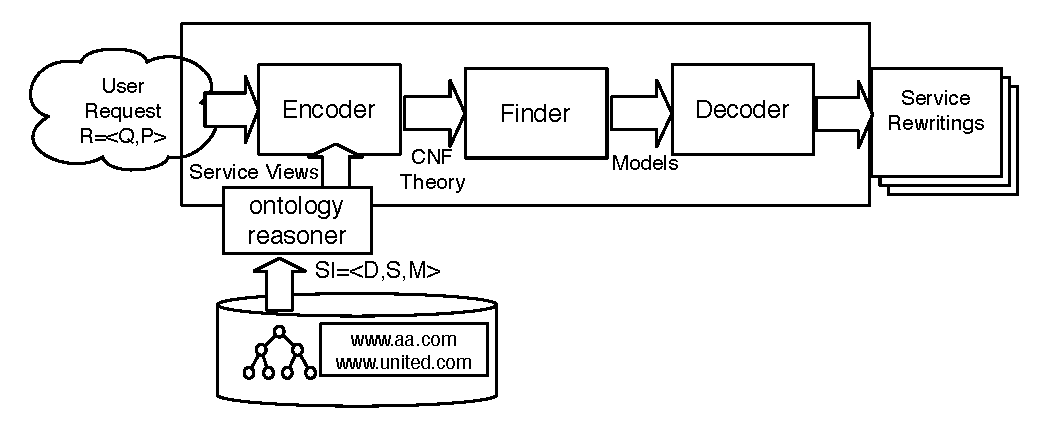
\includegraphics[width=.8\textwidth]{architecture}
\caption{System Architecture}
\label{fig:architecture}
\end{figure}

\Omit{
Once the CNF is generated, the compiler c2d, an off-the-shelf
component, compiles the CNF formula into d-DNNF.  A d-DNNF  theory is constructed from literals using only conjunctions  and disjunctions \cite{barwise:handbook}; for each conjunction its variables are pairwise disjoint, and for each disjunction, the disjuncts are pairwise logically contradictory; see Fig.~\ref{fig:dnnf} for an example.  In our approach, a d-DNNF theory is a compact representation of
all the rewritings. That is, the Finder generates in a backtrack-free
manner all the rewritings of the user request. If the user is interested in
a best rewriting, then the Finder computes it in
linear time in the size of the d-DNNF. If the user is interested in the 
all the best rewritings, these are computed in linear time in the
number of them. This computation transforms the DAG of the d-DNNF into a arithmetic
circuit by replacing the AND nodes with `+' and the OR nodes with `min'.
The literal ranking function assigns
values to the leaves of the circuit that are propagated to the
root in linear time. The value of the root is the rank of the
best model \cite{darwiche:weighted}.
Finally, if the user is interested in all rewritings,
these are also computed in linear time in the number of them.
In the latter two cases, if such number is exponential (in the size of the
input), the enumeration of the instantiations is also exponential but
this complexity is intrinsic to the problem and thus cannot be avoided.

It is important to remark
that the compilation process performed by the compiler c2d, needs to be performed only once as it does not
depend on the value of the QoS parameters or the user preferences. Thus, even if the compilation happens to be costly in terms of time, this cost can be amortized since the resulting
d-DNNF can be used to find best rewritings with respect to multiple values
of the QoS parameters or weights of user preferences.
Finally, the Decoder translates the best model returned by the Finder into
a rewriting that solves the SSP.

In order to make our results more accessible to a general audience, we decided
to present the experimental results in the next section, and leave the related work, and formal
and theoretical results for the following sections. In this way, the interested
reader may skip the formal details of the approach on a first reading.
}

\section{Experimental Results}

We conducted an empirical analysis on three benchmarks.
All the experiments were run on a desktop machine with an Intel
Core 2 Duo 2GHz CPU and 4Gb of memory, and the time was measured
with the Unix time command. We used the
compiler c2d, \footnote{\url{http://reasoning.cs.ucla.edu/c2d}} to compile 
the CNF formula into d-DNNF\cite{darwiche:weighted}; c2d makes use of
modern SAT techniques such as conflict-directed backtracking, clause learning
and caching\cite{darwiche:compiler} to enumerate the theory models from the d-DNNF.

The objective of the experiment is to assess the performance of the proposal
on varying conditions. The main benefit of our approach is that one can compile
the logical theory for a problem instance and then calculate all the instantiations,
or the best ones, any number of times. The cost model for finding best instantiations
can be changed with no need to recompile the logical theory. Therefore,
the time complexity of our approach is basically the time to encode the SSP
as a CNF plus the time to find the (best) models and the time to decode the
models. The times to encode and decode are negligible compared to the time to
enumerate the models. Because of this, we focus on the time to enumerate the
models of the benchmark problems. All the CNF theories are of low width.

The first benchmark consists of problems for air-travel queries.
Service views are of the form $V_i(x,y)\qrule\ \flight(x,y,\AL_i)$
where $\AL_i$ is a constant that denotes the name of an airline, 
and $\flight(x,y,\AL_i)$ relates the cities $x$ and $y$ such that
there is a flight between $x$ and $y$ served by $\AL_i$. This 
service is assumed to return all flights between two cities with an
specific airline. The user request has the form 
\[ Q(x_1,\ldots,x_n)\ \qrule\ \flight(\PA,x_1,z),\,\flight(x_1,x_2,z),\,\ldots,\,\flight(x_n,\NY,z)\,. \]

\begin{figure}[t]
\centering
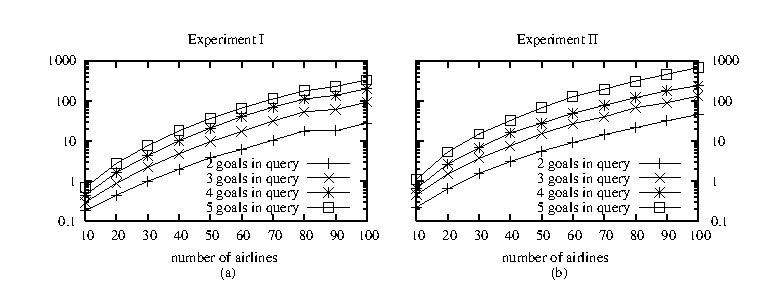
\includegraphics[width=1\textwidth]{plots/plot1}
\caption{Compilation times for experiments I and II for different
number of goals and different number of views. The plots are in
logarithmic scale, and the time is in seconds.}
\label{fig:plot1}
\end{figure}

The benchmark includes user requests with 2 to 5 sub-goals and
sets of 10 to 100 service views. The results for the compilation are
shown in panel (a) of Fig.~\ref{fig:plot1}. This is a plot in logarithmic
scale that suggests a sub-exponential behavior. In any case, the results
show good performance since realistic instances of the problem (sets of 100
airlines with 5-stop flights) can be compiled in 328 seconds.
The size in disk of the d-DNNF for 100 airlines and 5-stop flights is 3.4Mb.
On this d-DNNF, the best model can be computed in 0.29 seconds,
and the enumeration of all models in 0.47 seconds.

In an attempt to induce an exponential growth in the compilation time,
in the second benchmark we add a second service view for each airline.
This modification increases the number of valid rewritings from linear
to exponential since each leg of a flight can now be instantiated by two
services and thus a flight with $n$ legs may have up to $2^n$
rewritings.
We ran the compiler for instances comprising the same number of user request
sub-goals and total number of service views. The results plotted in
logarithmic scale are shown in panel (b) of Fig.~\ref{fig:plot1}.

These tests show good performance for this type of problems, but they do not
involve service views with multiple sub-goals. We therefore designed a
third experiment that consists unstructured, randomly generated instances.
Each instance contains three variables per domain ontology concept in the user request, ten distinct
variables and ten distinct constants, six sub-goals in the user request,
2 to 5 sub-goals in the service views, and a varying number of service views.
The chance that an argument of a domain ontology concept is bound to a constant is 50\%.
The results are depicted in Fig.~\ref{fig:plot4}.
The compilation time for these instances does not grow monotonically
since they are randomly generated. The same happens for the size of
the theories and the number of models. For example, the d-DNNF for 
a problem with 45 views each with 5 sub-goals is of size 5.1Mb and has
$1.26\times 10^8$ models. The time to find the best model for
this d-DNNF is 0.46 seconds while the time to enumerate all models
is about 17 hours.

\begin{figure}[t]
\centering
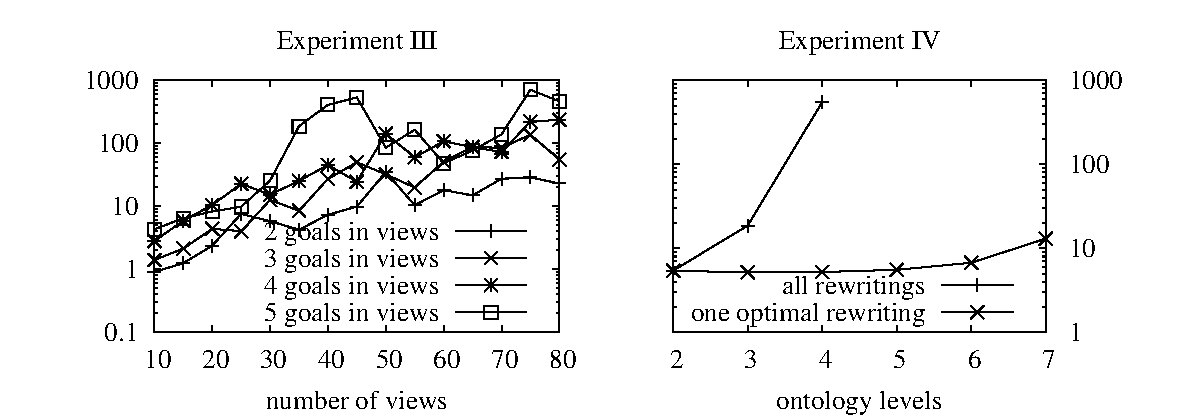
\includegraphics[width=.6\textwidth]{plots/plot4}
\caption{Compilation times for experiment III for different number of goals
and different number of views. Time for best rewriting for experiment IV. The plots are in logarithmic scale, and the time
is in seconds. }
\label{fig:plot4}
\end{figure}

These are preliminary experiments, yet the results show that the
proposed approach efficiently scales for problems with several goals
and views. We believe that these results are encouraging and motivate
us to continue this research. We plan to conduct additional experiments
with other types and sizes of user requests and, when possible, compare with
other approaches.


\section{Related Work}
The problem of selecting the services that satisfy a user request is a combinatorial
optimization problem and several heuristics have been proposed to find a good
solution in a reasonably short period of time~\cite{alrifaiR09,berardi08,myoung08,kuterG09,lecue09,rahmani08,sohrabiM09,Hiroshi2008}.

In a series of papers, Berardi and others~\cite{berardi05,berardi08,berardi06} 
describe services and workflows in terms of deterministic finite-state machines that are encoded using Description Logic theories whose models correspond to solutions of the problem; properties
of Description Logics reasoning methods are not exploited.

Ko et al.~\cite{myoung08} propose a constraint-based approach that encodes the nonfunctional
permissible values as a set of constraints whose violation needs to be
minimized. Alrifai and Risse~\cite{alrifaiR09} develop a two-fold solution that uses a hybrid
integer programming algorithm to find the decomposition of global QoS into local
constraints, and then, selects the services that best meet the local constraints.

Recently, two planning-based approaches have been proposed. Kuter and
Golbeck~\cite{kuterG09} extend the SHOP2 planning algorithm to select the trustworthy
composition of services that implement a given OWL-S process model, while
Sohrabi and McIlraith~\cite{sohrabiM09} propose a HTN planning-based solution where user
preference metrics and domain regulations are used to guide the planner into
the space of relevant compositions. Finally, L\'ecu\'e \cite{lecue09}  develops a genetic-based
algorithm to identify the composition of services that best meet the quality
criteria for a set of QoS parameters.

These existing solutions are able to scale up to relatively large number of
abstract concepts. In addition to scalability, our approach provides a more expressive
framework where services are semantically described in terms of domain
ontology concepts, user preferences restrict the space of solutions, and ontology
relationships augment the space of possible solutions. Finally, our approach
is sound and complete.

\Omit{
\subsection{Query Rewriting}

A number of algorithms have been developed to find the rewritings of a given query;
the most prominent being the Bucket algorithm \cite{levy:bucket}, the Inverse Rules
algorithm \cite{pods:DuschkaG97,Qian96}, the \minicon\ algorithm \cite{pottinger:minicon},
and the \mcdsat\ algorithm \cite{arvelo:aaai06}.
Generally, query rewriting algorithms work in two phases. During the first phase,
the algorithms identify the views that rewrite at least one sub-goal of the query, and
during the second, these partial rewritings are combined into complete rewritings.
The main difference between the algorithms is the criteria used to choose the relevant
views to reduce the space of non-useful rewritings.

The Bucket algorithm reduces the number of possibilities by just considering each
sub-goal in the query in isolation, and selecting the views that are able to produce
at least the attributes projected by the query. Since the attributes involved in the
joins in the query are not verified, a large number of rewritings comprised of Cartesian
products may be generated. 	

The Inverse Rules algorithm constructs a set of rules that invert the view definitions
and establish how to compute tuples for the database relations from the tuples of the
views. Similarly to the Bucket algorithm, it can produce a large number of non-useful
rewritings. 

The \minicon\ algorithm overcomes the limitations of the previous algorithms by identifying
only views that rewrite a set of the sub-goals of the query, and that can be combined with
the rest of the sub-goals. The key idea is to identify the mappings between the variables in
each sub-goal to the variables in one or more sub-goals in the views, in a way
that join variables in the query are mapped to join variables in the body of a view or to
the distinguished variables of the view. Mappings between variables and sub-goals are
represented in the so-called MiniCon Descriptions (MCDs) \cite{pottinger:minicon}.

Finally, the \mcdsat\ algorithm is able to identify the query rewritings of a query by
translating the problem of rewriting into the problem of enumerating the models of a
propositional theory whose models are in correspondence with the rewritings of the query.
The algorithm exploits the properties of d-DNNFs to efficiently enumerate the models of
the theory.
The \mcdsat\ algorithm has demonstrated to scale better than the \minicon\ algorithm over
a large number of benchmarks often showing performance improvements of several orders of
magnitude. However, the \mcdsat\ algorithm was not designed for rewriting problems
involving explicit constants, nor to compute the best rewritings with respect to a given
utility function or user preferences. We propose an extended encoding that 
overcomes these limitations and apply the encoding to SSP.

\subsection{Knowledge Compilation}

Knowledge compilation is the area in AI concerned with the problem of mapping
logical theories into suitable fragments that make certain desired operations
tractable \cite{cadoli:compilation}. Different compilation languages have been
defined, for instance, Ordered Binary Decision Diagrams (OBDDs) \cite{bryant:obdd},
Negation Normal Form (NNF) \cite{barwise:handbook}, and Decomposable Negation
Normal Form (DNNF) \cite{darwiche:map}. In this work, we make use of the properties
of the deterministic DNNFs (d-DNNF) \cite{darwiche:d-dnnfs} to provide an scalable
and efficient solution to the Service Selection Problem. 

A Negation Normal Form (NNF) theory is constructed from literals using only conjunctions
and disjunctions \cite{barwise:handbook}. An NNF is said to be decomposable (DNNF) \cite{darwiche:d-dnnfs} if for each conjunction, its variables are pairwise disjoint. A DNNF is said to be deterministic (d-DNNF) \cite{darwiche:d-dnnfs} if for each disjunction, the disjuncts are pairwise logically contradictory. A d-DNNF supports model counting in polytime in the size of its DAG, and model
enumeration in polytime in the size of the output.
Furthermore, given a literal ranking function $r$, one can compute the rank
of the best model in polytime for DNNFs \cite{darwiche:weighted}.

The fragments DNNF and d-DNNF are universal yet translating a CNF theory 
to DNNF format has an exponential cost in the worst case. This translation
is referred to as compilation in the field. There is a publicly available
compiler, called c2d,\footnote{\url{http://reasoning.cs.ucla.edu/c2d}}
that performs this compilation process and that makes
use of modern SAT techniques such as conflict-directed backtracking,
clause learning and caching \cite{darwiche:compiler}.
This compiler incurs in the worst case in exponential space in a parameter
called the width of the decomposition tree that is related to the ``connectivity''
of the CNF theory. However, in our experiments, the CNF theories that are
compiled are of low width.

\section{SSP Formalization into Logical Theories}
We use an approach similar to the one described in \cite{arvelo:aaai06} to
encode the SSP. We have limited space to make a comprehensive description of
the logical theory so the reader is referred there for details and formal results.

We identify service compositions  by enumerating the models of a logical
theory $\Delta=\Delta_{com}\cup\Delta_{id}^1\cup\cdots\Delta_{id}^N$
where $\Delta_{com}$ specifies how to combine $N$ independent copies theories
$\Delta_{id}$ that cover the goals in a user request $Q$.
Each $\Delta^i_{id}$ is a tagged copy $\Delta_{id}$ in which each literal
$\ell$ is tagged as $\ell^i$.
The Instantiation Description (ID) theory $\Delta_{id}$ consists of different
groups of clauses that guarantees that its models are in correspondence with
partial rewritings, while the theory $\Delta_{com}$ contains additional
clauses to guarantee a sound and complete combination of partial rewritings
into a complete rewriting.
The ID theory $\Delta_{id}$ consists of the following variables:
\begin{enumerate}[--]
\item $\{v_0,\ldots,v_n\}$ to indicate which source view $V_i$ is used, or $v_0$ to indicate the null ID.
\item $\{g_1,\ldots,g_m\}$ to indicate the goals covered by the view.
\item $\{z_{j,k,i}\}$ to indicate that the $j$th goal in $Q$ is covered by the $k$th goal in $V_i$.
\item $\{t_{x,y}\}$ to indicate that the variable/constant $x$ in $Q$ is mapped into the
      variable/constant $y$ in the view.
\end{enumerate}
The ranges of the indices for the $z$ and $t$ variables depend on the problem.

The following clauses encode the SSP problem in terms of the LAV mappings in $M$.
Rajaraman et al.\ \cite{RajaramanSU95} showed that for queries without negation or
arithmetic comparisons, but with constants, and $m$ goals and $k$ variables in the
head of the user request, it is enough to consider rewritings of length at most $N=m+k$.
\begin{enumerate}[C10.]
\item[C1.] (At least one view is used): $\bigvee_{i=0}^n v_i$.
\item[C2.] (At most one view is used): $\neg v_i\lor\neg v_j$ for $i\neq j$.
\item[C3.] (Null view equals null): $v_0 \Rightarrow \neg g_j$ for $1\leq j\leq m$.
\item[C4.] (Views are useful): $v_i \Rightarrow \bigvee_{j=1}^m g_j$ for $1\leq i\leq n$.
\item[C5.] (Subgoals covered at most once): $z_{j,k,i} \Rightarrow \neg z_{j,l,i}$ for appropriate $i,j,k,l$.
\item[C6.] (Scope of views): $v_i \Rightarrow \neg g_j$ for goals that cannot be covered by $V_i$.
\item[C7.] (Consistency): $v_i \land g_j \Leftrightarrow \bigvee z_{j,k,i}$ for appropriate $i,j,k$.
\item[C8.] (Dead variables): $v_i \Rightarrow \neg t_{x,y}$ for all $x,y$ with $y\notin V_i$.
\item[C9.] (1-1 for $\exists$ vars): $v_i \land t_{x,y} \Rightarrow \neg t_{x,y'}$ for all
           existential variables $y,y'\in V_i$.
\item[C10.] (Distinguished): $v_i \Rightarrow \neg t_{x,y}$ for distinguished $x$ and existential
            $y\in V_i$.
\item[C11.] (Existential): $v_i\land t_{x,y}\Rightarrow g_j$ for exist.\ $y\in V_i$ and
            goals $g_j$ that contain $x$.
\item[C12.] (Match): $v_i\land z_{j,k,i} \Rightarrow t_{x,y}$ for all $x,y$ that must match
            if $g_j$ is covered by goal $k$ in $V_i$.
\item[C13.] (If all vars in $V_i$ are distinguished, it covers only one goal):
            $v_i \land g_j \Rightarrow \neg g_k$ for appropriate views $v_i$.
\end{enumerate}
These clauses are the same clauses used by \mcdsat\ to encode QRPs \cite{arvelo:aaai06}.
In order to properly manage constant symbols, the clauses must be enhanced with:
\begin{enumerate}[C10.]
\item[C14.] (Direct inconsistency 1): $t_{x,A} \Rightarrow \neg t_{x,B}$.
\item[C15.] (Direct inconsistency 2): $t_{A,x} \Rightarrow \neg t_{B,x}$.
\item[C16.] (Direct inconsistency 3): $\neg t_{A,B}$.
\item[C17.] (Transitivity 1): $v_i\land t_{A,y}\land t_{x,y}\land t_{x,z}\Rightarrow t_{A,z}$.
\item[C18.] (Transitivity 2): $v_i\land t_{y,A}\land t_{y,x}\land t_{z,x}\Rightarrow t_{z,A}$.
\end{enumerate}
Recall that, as shown in Section~2, the main issue when handling
constants is to be sure that not two different constants are mapped
into each other either directly or indirectly.
Clauses C14--C16 prune direct inconsistent mappings, while the last
two clauses implement a restricted propagation of mappings that prune
indirect inconsistencies.
Likewise, the theory $\Delta_{com}$ that specifies complete
instantiations contains the following clauses:
\begin{enumerate}[C10.]
\item[C19.] (Cover all goals): $\bigvee_{j=1}^m g^i_j$ for $1\leq i\leq N$.
\item[C20.] (Disjunctive cover): $g^i_k \Rightarrow \neg g^j_k$ for $i\neq j$.
\item[C21.] (Prune symmetries): $g^i_j \Rightarrow \bigvee_{k=1}^{j-1} g^{i-1}_k$
            for $1\leq j\leq m$ and $1\leq i\leq N$.
\item[C22.] (Direct inconsistency 4): $t^i_{x,A} \Rightarrow \neg t^j_{x,B}$.
\end{enumerate}
These clauses provide a sound and complete characterization of SSPs in the
sense that their models are in correspondence with the rewritings of the user request.

For the QoS parameters, we assume a simple additive aggregation model in
which each view $V_i$ is associated with a cost $c(V_i)$ (negative if utility),
and a complete rewriting with the sum of the cost of its views. User preferences rules are transformed into propositional logic formulas whose cost is a high number.
An optimal or best solution is one with minimum cost, and the
optimal value of the SSP is the cost of an optimal rewriting.
A SSP always has a well-defined optimal value (if there are no rewritings,
its cost is $\infty$), but it may have multiple best rewritings.
The SSP with costs consists in finding all optimal rewritings or
one rewriting, this depends on the particular application.
In our formulation, this can be done from the d-DNNF that encodes $\Delta$
using the literal ranking function $r$ that assigns $r(\ell)=c(V_i)$ if
$\ell=v_i$, and $r(\ell)=0$ if $\ell\notin\{v_1,\ldots,v_n\}$.
}
\section{Conclusions and Future Work}
We have shown how the propositional theory used in \mcdsat\  for computing
rewritings of queries can be extended to efficiently encode SSP and by exploiting
known properties of modern SAT solvers, we provide an efficient and scalable
solution to SSP. In addition, we provide an expressive framework defining LAV
mappings to semantically describe services, and expressing user requests as a
conjunctive query over the domain ontology concepts and a set of preferences
that restrict the SSP solutions.

The experimental results show that the approach can be applied to real-sized
problems; however, if d-DNNF format is used, the approach is only possible
when the compilation of the CNF theory into d-DNNF format succeeds. Thus,
to overcome this limitation, in the future, we plan to study the performance
and scalability of our approach in other off-the-self model enumeration and SAT
solvers such as Relsat, Minisat and MiniMaxSAT. We also are interested in using
other target compilation languages like Ordered Binary Decision Diagrams.

\bibliographystyle{abbrv}
\bibliography{ref}

\end{document}

